\chapter{Evolutionary dataset optimisation}
\label{chp:edo}

\graphicspath{{chapters/edo/paper/img/}}
\renewcommand{\tikzpath}{chapters/edo/paper/tex/diagrams}
\renewcommand{\algpath}{chapters/edo/paper/tex/algorithms}

\begin{center}
    The research reported in this chapter has led to a
    publication~\cite{Wilde2020:edo} entitled:\\[1em]

    {%
        \bf\itshape{``Evolutionary dataset optimisation: learning algorithm
                    quality through evolution''}
    }

    Available online at:~\doi{10.1007/s10489-019-01592-4}\\
    Associated data:~\doi{10.5281/zenodo.3492228}\\
    Source code:~\doi{10.5281/zenodo.3492236}\\[1em]

    The abstract of the publication is as follows:\\[1em]
\end{center}

In this paper we propose a novel method for learning how algorithms perform.
Classically, algorithms are compared on a finite number of existing (or newly
simulated) benchmark datasets based on some fixed metrics. The algorithm(s) with
the smallest value of this metric are chosen to be the `best performing'. We
offer a new approach to flip this paradigm. We instead aim to gain a richer
picture of the performance of an algorithm by generating artificial data through
genetic evolution, the purpose of which is to create populations of datasets for
which a particular algorithm performs well on a given metric. These datasets can
be studied so as to learn what attributes lead to a particular progression of a
given algorithm. Following a detailed description of the algorithm as well as a
brief description of an open source implementation, a case study in clustering
is presented. This case study demonstrates the performance and nuances of the
method which we call Evolutionary Dataset Optimisation. In this study, a number
of known properties about preferable datasets for the clustering algorithms
known as \(k\)-means and DBSCAN are realised in the generated datasets.

\myrule%

The differences between this chapter and the publication are an extended
discussion of the motivation behind the Evolutionary Dataset Optimisation method
(in Section~\ref{sec:edo:intro}) and its components
(Section~\ref{sec:algorithm}), as well as a revised case study which concludes
the chapter (Section~\ref{sec:examples}).

The source code used to generate the plots and datasets in this chapter have
been archived online under \doi{10.5281/zenodo.4000316}. The datasets themselves
have been archived under \doi{10.5281/zenodo.4000327}.

\section{Introduction}\label{sec:edo:intro}

This chapter introduces a novel method called Evolutionary Dataset Optimisation
(EDO). At its core, EDO is an evolutionary algorithm that acts on datasets to
optimise some real-valued function. While it is possible to perform classical
optimisation tasks with this method, its primary application is in learning the
quality of an algorithm. The concept of an algorithm's quality here refers to
some combination of its robustness, and its strengths and weaknesses.

When developing an algorithm to solve a given problem, questions are raised
about its performance, both objectively and relative to existing methods.
Determining convincing answers to these questions is an inherently difficult
task. However, under the current regime, there is a standard response: take 
benchmark datasets and a common metric (or set thereof) amongst the proposed
method, and its competitors, then assess the methods based on this metric and
deem those with the smallest value to be `best'.

Objectively, there is nothing wrong about comparing methods in this way except
for the semantics of the outcome, i.e. outperforming a method on a dataset with
a metric is insufficient evidence to categorise one method as `better' than
another. Each case can be qualified with something along the lines of ``Method
\(A\) performs better than Method \(B\) under the given conditions'', but there
are concerns about this process that persist beyond linguistic hair-splitting. 

A significant concern presented by this process is in how benchmark examples are
selected; there is no real measure of their reliability other than their
frequent use. There do exist benchmark dataset suites that are curated to be
relevant, diverse and comprehensive for some problem domains --- such as machine
learning~\cite{Dua2019,Olson2017} and time series~\cite{UCRArchive2018} --- but
it is often the case that a dataset becomes a benchmark for merely being
long-standing and used many times. This title awards the dataset with the
accolades of being reliable and trustworthy. However, this is not guaranteed.

Computer vision is one such domain where these questionable de facto benchmarks
have come to exist. In~\cite{Prabhu2020}, the authors dissect the unethical and
problematic practices used in the creation and aggregation of several benchmark
datasets from computer vision, including the renowned \emph{ImageNet}
datasets~\cite{Deng2009}. These practices pose serious questions about the
credibility of the models trained using these benchmarks, both morally and as a
matter of their performance. The exposition highlights questions of consent and
privacy as well as revealing a valid moral quandary given that the social,
cultural and racial biases transferred from these datasets to the models will
then diffuse into systems that are synonymous with life in the age of `Big
Data'.

As an example of the reality of these systemic biases, in 2015, it was made
public that the automatic classifier developed as part of \emph{Google Photos}
had been incorrectly labelling images of people of colour as gorillas. Google
publicly apologised and vowed to fix the problem, but since then the only action
taken to mitigate this has been to remove several primates from the set of
labels available to their model~\cite{Simonite2018}.

Leaving computer vision aside, the authors of \cite{Campos2016} raise questions
about the availability and suitability of benchmark datasets in the field of
unsupervised outlier detection. The authors point out that even though
systematic approaches exist for the generation of benchmark datasets, the
approaches are not sufficiently documented to be reproducible, thus rendering
them scientifically moot.

In addition to this, the authors discuss the troubles that come with co-opting
datasets designed for another task (classification in their case) in the absence
of existing benchmarks designed for outlier detection. This practice is
indicative of another issue with this aspect of the current paradigm where
convenience has become a driving force for benchmark selection rather than
merit.

Striving for convenience may well be an issue that stems from the competitive
nature of algorithm design. In order for a method to become `state-of-the-art',
there has to be some comparable evaluation with existing methods. However, this
should not be the end of the line when discussing the quality of any method.
More extensive work is required to understand an algorithm truly and to quantify
its quality, which leads to the other source of concern in the established
process: the methods themselves.

Holding a method to account on a finite number of example datasets ---
regardless of their reliability or diversity --- limits the amount of learning
one can gain about that method. In particular, it limits the understanding of
the characteristics which lead to good or bad performance to those attributes
present in the set of example datasets. Another example from computer
vision~\cite{Torralba2011} shows that Support Vector Machines (SVMs) --- the
use of which is ubiquitous in classification --- fail to perform well when
tested on a dataset containing comparable and broadly equivalent items to the
one on which they have been trained. So, despite the abundant use of SVMs, even
in the then-`best' image classifier, there should be concerns about the
robustness of the model.

Taking a step back from examples of empirical algorithm evaluation, consider the
space between algorithms and data more generally. To evaluate an
algorithm,~i.e.\ a fixed point in the space of algorithms, one maps it to a
finite subset of points in the space of datasets using some metric(s). How that
subset is determined is what has been discussed thus far. The process when
travelling in the opposite direction is not so standardised, but it appears more
rigorous.

Suppose that the object of interest was not an algorithm but rather a dataset.
In this case, the objective is to determine a preferable algorithm to complete
some task on the data. There exist many ways of achieving this that appear in a
range of disciplines. However, each takes into account the constraints and
characteristics of the data and the context of the research problem. These
methods are often equivalent to asking questions of the data and can include the
use of diagnostic tests. For instance, in the case of clustering, if the data
displayed an indeterminate number of non-convex blobs, then one could recommend
that an appropriate clustering algorithm would be DBSCAN~\cite{Ester1996}.
Otherwise, for scalability, \(k\)-means may be chosen~\cite{Wu2009,Zhao2009}.

The EDO method belongs to a new paradigm that aims to flip the process described
here by allowing the data itself to be unfixed. EDO achieves this fluidity by
generating data for which the algorithm of interest performs well (or better
than some other) through the use of an evolutionary algorithm (EA). The purpose
of doing so is not only to create a bank of useful datasets, but rather to allow
for the subsequent studying of those datasets. Undergoing this study reveals the
attributes and characteristics which lead to the success (or failure) of the
algorithm, giving a broader understanding of the algorithm on the whole.
Figure~\ref{fig:paradigm} provides a diagram of this framework. On the right:
the current path for selecting some algorithm(s) based on their validity and
performance for a given dataset; on the left: the proposed flip to better
understand an algorithm by exploring the space in which `good' datasets exist
for that algorithm.

\inputtikz{paradigm}{%
    A diagram of the current and proposed paradigms for algorithm evaluation
}

As will be seen later in this chapter, the most substantial limitation of this
paradigm is in defining a meaningful fitness function for the EA.
Section~\ref{sec:examples} acts as a tutorial on how to resolve this issue
using an iterative approach where the fitness function is adjusted so as to
avoid redundant, trivial or reductive results. Although the case study in that
section of this chapter focuses on clustering, the generic form of the EA means
that any method which acts on tabular data is suitable for study using EDO.

It is also important to note that the method described in this chapter is merely
one element of this new paradigm, and is one that utilises evolution. EAs have
been applied successfully to solve a wide array of problems --- particularly
where the complexity of the problem or its domain is significant. These methods
are highly adaptive, and their population-based construction (displayed in
Figure~\ref{fig:flowchart}) allows for the efficient solving of problems that
are otherwise beyond the scope of traditional search and optimisation methods.
An EA approach has been chosen here as they are uncomplicated in design, yet
their capabilities encompass the difficulties of the flipped paradigm set out
above.

\inputtikz{flowchart}{%
    A general schematic for an evolutionary algorithm
}

The use of EAs to generate artificial data is not a new concept, however.
Applications of EAs to data generation have included developing methods for the
automated testing of software~\cite{Koleejan2015,Michael2001,Sharifipour2018}
and the synthesis of existing or confidential data~\cite{Chen2016synthetic}.
Such methods also have a long history in the parameter optimisation of
algorithms, and recently in the automated design of convolutional neural network
(CNN) architecture~\cite{Suganuma2017,Sun2018}.

Other methods for the generation or synthesis of artificial data are numerous
and range from simple concepts such as simulated annealing~\cite{Matejka2017} to
swarm-based learning techniques~\cite{Abualigah2018b} or generative adversarial
networks (GANs)~\cite{Goodfellow2014}. The unconstrained learning style of
methods like CNNs and GANs aligns with those in the proposed paradigm, and with
EDO in particular. By allowing the EA to explore and learn about the search
space in an organic way, an unprejudiced insight can be established that is not
necessarily reliant on any particular framework or agenda.

Note that there is no necessary restriction on the search space to be of a fixed
dimension or data type such as the method described in~\cite{Chen2016synthetic}.
The shape of a dataset is considered a part of the search space itself that can
be traversed through the EA.

The remainder of this chapter is structured as follows:

\begin{itemize}
    \item Section~\ref{sec:algorithm} describes the parameterisation, structure
        and components of the EDO method.
    \item Section~\ref{sec:examples} contains a case study examining the success
        and failure of \(k\)-means clustering using EDO. Included also is a
        comparison between \(k\)-means and another clustering algorithm DBSCAN.\
    \item Section~\ref{sec:edo:summary} summarises the chapter.
\end{itemize}

In addition to the case study at the end of this chapter, the EDO method is
instrumental in evaluating the algorithm presented in Chapter~\ref{chp:kmodes}.

\section{The evolutionary algorithm}\label{sec:algorithm}

This section presents the details of the EDO algorithm. As stated previously,
the EDO method is an EA. The EA follows a typical schema with the addition of
some features that align with the overall objective of artificial data
generation. With that, there are a number of parameters that are passed to EDO.
These include the typical parameters of an evolutionary algorithm: a fitness
function, \(f\), which maps from an individual to a real number (or some
quantity which can be ordered), a population size, \(N \in \mathbb N\), a
maximum number of iterations, \(M \in \mathbb N\), a selection parameter, \(b
\in [0, 1]\), and a mutation probability, \(p_m\).

In addition to these, EDO takes a number of parameters which allow the EA to act
on datasets of varying sizes and forms. The required parameters are as follows:

\begin{itemize}
    \item A set of probability distribution families, \(\mathcal{P}\). Each
        family in this set has some parameter limits which form a part of the
        overall search space. For instance, the family of normal distributions,
        denoted by \(N(\mu, \sigma^2)\), would have limits on values for the
        mean, \(\mu\), and the standard deviation, \(\sigma\).
    \item A maximum number of \emph{subtypes} for each family in
        \(\mathcal{P}\). A subtype is an independent copy of the family
        distribution that progresses separately from the other subtypes in that
        family. These are the actual distribution objects which are traversed in
        the optimisation and that are passed to the individuals.
    \item A probability vector to sample distributions from \(\mathcal{P}\),
        \(w = \left(w_1, \ldots, w_{|\mathcal{P}|}\right)\).
    \item Limits on the number of rows an individual dataset can have,
        \vspace{-1ex}\[
            R \in \left\{%
                (r_{\min}, r_{\max}) \in \mathbb{N}^2~|~r_{\min} \leq r_{\max}
            \right\}
        \]\vspace{-2em}
    \item Limits on the number of columns a dataset can have,
        \vspace{-1ex}\[
            C := \left(C_1, \ldots, C_{|\mathcal{P}|}\right)
            \text{ where }
            C_j \in \left\{ (c_{\min}, c_{\max}) \in {%
                \left(\mathbb{N}\cup\{\infty\}\right)
            }^2~|~c_{\min} \leq c_{\max}\right\}
        \]
        for each \(j = 1, \ldots, |\mathcal{P}|\). That is, \(C\) defines the
        minimum and maximum number of columns a dataset may have from each
        distribution in \(\mathcal{P}\).
\end{itemize}

The remaining two parameters are optional, but can be useful for introducing and
focusing exploration, respectively:

\begin{itemize}
    \item A second selection parameter, \(l \in [0, 1]\), to allow for a
        small proportion of `lucky' individuals to be carried forward.
    \item A shrink factor, \(s \in [0, 1]\), defining the relative size of a
        component of the search space to be retained after adjustment.
\end{itemize}

Choosing an optimal set of parameters for any given run of EDO is not concrete
--- as is the case with all EAs --- and some experimentation may be required.
For the dataset-specific parameters --- like \(\mathcal P\), \(R\), and \(C\)
--- these decisions are practical in nature for the most part. Large datasets
(controlled by \(R\) and \(C\)) will require more computational power and
storage, for instance. For the EA-specific parameters, there are some rules of
thumb such as:

\begin{itemize}
    \item Choosing a population size, \(N\) large enough to take a
        representative sample from the search space. \(N=100\) is a good
        starting point, but larger populations should provide better samples.
    \item Setting the selection pressure, \(b\), so as to encourage the
        preservation of favourable characteristics in the individuals, and not
        to dilute the next population. Typical values for achieving this with
        other EAs range between \(0.1\) and \(0.25\).
    \item Including enough mutation (through \(p_m\)) to force some
        heterogeneity in the population and to further explore the search space.
        However, heavy-handed mutation will likely cause the EA to diverge,
        leading to reductive results. Typical mutation probabilities are between
        \(0.01\) and \(0.05\).
\end{itemize}

Algorithm~\ref{alg:edo} provides a high-level description of the EDO algorithm,
presenting its general structure. This section comprises more detailed
discussion --- along with relevant examples, diagrams and algorithm statements
--- for the processes mentioned there: the creation of individuals, the
evolutionary operators and the `shrinkage' process. In addition, an overview of
a software implementation is provided.

\inputalg{edo}
\inputalg{new_population}

Note that there are no defined processes for how to stop the algorithm or adjust
the mutation probability, \(p_m\), in this chapter. This generality is
deliberate and is down to the particular use case. Some examples include:

\begin{itemize}
    \item Regular decreasing in mutation probability across the available
        attributes~\cite{Kuehn2013}.
    \item Stopping when no improvement in the best fitness is found within some
        \(K\) consecutive iterations~\cite{Leung2001}.
    \item Utilising global behaviours in fitness to indicate a stopping
        point~\cite{Marti2016}.
\end{itemize}


\subsection{The software implementation}

The remainder of this section discusses the components and mechanisms of the EDO
method in a largely mathematical manner. However, a Python implementation of EDO
has been developed as part of this thesis, \edo. The software is freely
available online under the Massachusetts Institute of Technology (MIT) licence,
and can be found hosted on GitHub (at~\github{daffidwilde/edo}) or archived on
Zenodo (at~\doi{10.5281/zenodo.2552890}). Furthermore, \edo\ is registered on
the Python Package Index and can be installed through standard Python practices,
including via \pip\ --- as in Snippet~\ref{snp:edo-pip}.

\begin{listing}[htbp]
\begin{usagesh}
> pip install edo
\end{usagesh}
\caption{Installing the \edo\ library via \pip}\label{snp:edo-pip}
\end{listing}

The \edo\ library is built on the scientific Python stack~\cite{pandas,numpy}
and has been developed to be consistent with the current best practices of
open-source software development; these are discussed in
Section~\ref{sec:dev}. As such, the software is modular, automatically tested
and fully documented. The documentation for \edo\ is available at
\url{edo.readthedocs.io}, and Figure~\ref{fig:docs} contains a screenshot of one
of the tutorial pages.

\graphicspath{{./}}
\begin{figure}[htbp]
    \centering
    
\includegraphics[width=\imgwidth]{img/docs.png}
    \caption{A screenshot of one of the \edo\ library tutorials}
    \label{fig:docs}
\end{figure}

In Section~\ref{sec:examples}, the \edo\ implementation is used to carry out an
investigation into \(k\)-means clustering. The tutorial shown in
Figure~\ref{fig:docs} is a simplified version of the example in
Section~\ref{subsec:inertia}. Given the size and number of examples in the
closing section of this chapter, a command-line tool, \edolab, is used to run
the experiments. To demonstrate how \edo\ should be used directly, consider the
following scenario.

Let \(X\) be a dataset with two columns, \(X_r\) and \(X_a\), which each contain
\(n \in [50, 100]\) real values. The values of \(X_a\) are drawn uniformly from
the interval \([-2\pi, 2\pi]\), while those in \(X_r\) may take values from the
interval \([0, 2]\). Again, these values are sampled uniformly.

The objective is to find a dataset, \(X\), which maximises the following
function:

\begin{equation}\label{eq:circle}
    f(X) = \frac{\text{Var}\left(X_{a}\right)}{%
        \max_{x \in X_r} \left|x - 1\right|%
    }
\end{equation}

That is, to find a dataset with maximal variance in one column, and minimal
maximum distance from one in the other. Such a dataset would describe the polar
coordinates of some set of points along the unit circle. The points in
\(X_r\) correspond to the radii, and those in \(X_a\) correspond to the angle
from the origin in radians.

The first step in implementing this scenario in \edo\ is to choose appropriate
distribution classes. These classes go on to form the families in EDO,
\(\mathcal P\). The \edo\ documentation includes detailed instructions on how to
implement new distribution classes
(\href{https://edo.readthedocs.io/en/latest/how-to/new_column.html}{%
\nolinkurl{edo.readthedocs.io/.../how-to/new\_column.html}}), but several
common distributions are already implemented; these include the uniform
distribution. Since both \(X_r\) and \(X_a\) sample their values uniformly and
from different bounds, separate subclasses of the
\mintinline{console}{edo.distributions.Uniform} class must be created.
Snippet~\ref{snp:uniforms} shows how this should be done.

\begin{listing}[htbp]
\begin{usagepy}
>>> import numpy as np
>>> from edo.distributions import Uniform
>>> 
>>> class RadiusUniform(Uniform):
...     """A uniform distribution for radii"""
...     name = "RadiusUniform"
...     param_limits = {"bounds": [0, 2]}
>>> 
>>> class AngleUniform(Uniform):
...     """A uniform distribution for angles"""
...     name = "AngleUniform"
...     param_limits = {"bounds": [-2 * np.pi, 2 * np.pi]}

\end{usagepy}
\caption{An \edo\ implementation for separate uniform distribution classes}
\label{snp:uniforms}
\end{listing}

With the column distributions implemented, the fitness function needs defining.
Snippet~\ref{snp:fitness} contains the code to implement the fitness function
given in~\eqref{eq:circle}. Since each column of the dataset is of a specific
type, they must be recovered properly; this is done using the
\mintinline{console}{split_individual} function.

\begin{listing}[htbp]
\begin{usagepy}
>>> def split_individual(individual):
...     """ Separate the columns of an individual's dataframe. """
...     df, metadata = individual
...     names = [m.name for m in metadata]
...     radii = df[names.index("RadiusUniform")]
...     angles = df[names.index("AngleUniform")]
...     return radii, angles
>>> 
>>> def fitness(individual):
...     """ Determine the similarity of the dataset to the unit circle. """
...     radii, angles = split_individual(individual)
...     return angles.var() / (radii - 1).abs().max()

\end{usagepy}
\caption{Implementing the circle fitness function in \edo}
\label{snp:fitness}
\end{listing}

Now all the required components are ready, the EDO algorithm can be run
using the \mintinline{console}{edo.DataOptimiser} class.
Snippet~\ref{snp:circle} shows the code required to run the EDO algorithm on
this scenario across several random seeds. These seeds make the runs repeatable,
and their outputs reproducible.

\begin{listing}[htbp]
\begin{usagepy}
>>> import edo
>>> import pandas as pd
>>> 
>>> pop_histories, fit_histories = [], []
>>> for seed in range(5):
...     families = [edo.Family(RadiusUniform), edo.Family(AngleUniform)]
...     opt = edo.DataOptimiser(
...         fitness,
...         size=100,
...         row_limits=[50, 100],
...         col_limits=[(1, 1), (1, 1)],
...         families=families,
...         max_iter=30,
...         best_prop=0.1,
...         maximise=True,
...     )
...     pops, fits = opt.run(random_state=seed)
...     fits["seed"] = seed
...     pop_histories.append(pops)
...     fit_histories.append(fits)
>>> 
>>> fit_history = pd.concat(fit_histories)

\end{usagepy}
\caption{Running the circle scenario in \edo\ across five seeds}
\label{snp:circle}
\end{listing}

Here, the remaining parameters --- population size, selection parameters, etc.
--- are mainly illustrative and such that this example can run in good time.
However, despite this potential roughness, the results are good.
Figure~\ref{fig:circle} shows a contour of the top 50\% of individuals, which is
well-distributed about the unit circle. In addition, the best-performing
individual from across these runs is shown as a scatter.

\begin{figure}
    \centering
    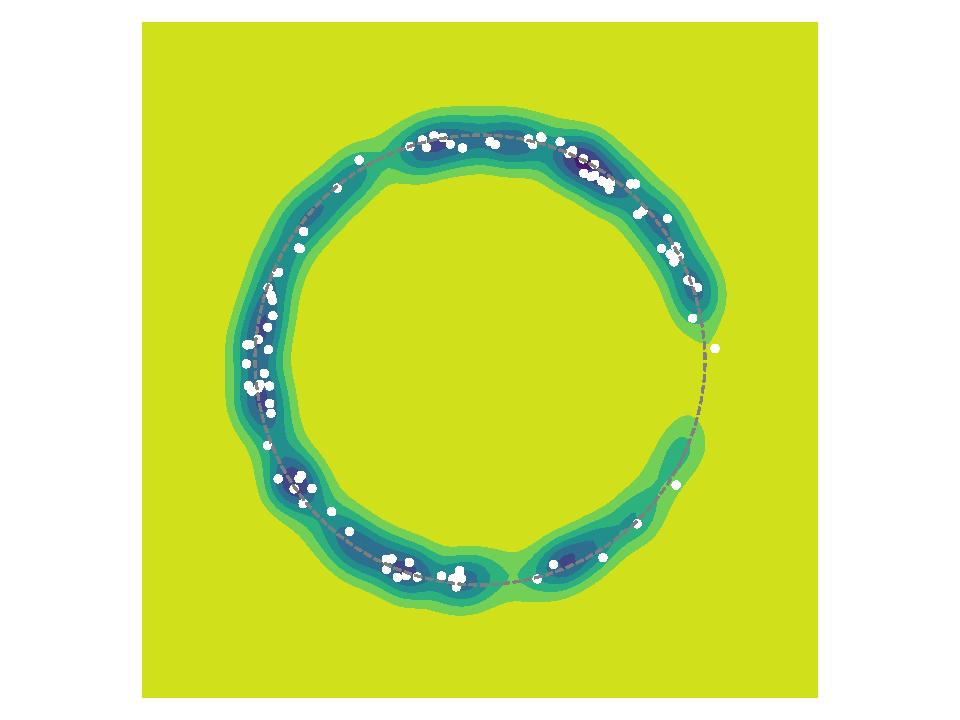
\includegraphics[width=\imgwidth]{img/circle/main}
    \caption{A contour and scatter plot of the circle example results}
    \label{fig:circle}
\end{figure}
\graphicspath{{chapters/edo/paper/img/}}

\subsection{Individuals}

Evolutionary algorithms operate in an iterative process. At each iteration, the
EA acts on a population (generation) of \emph{individuals}. Each individual
corresponds to a solution to the problem in question according to some
representation or encoding. In a genetic algorithm, an individual is a solution
encoded as a bit string of typically fixed length and is treated as a
chromosome-like object to be manipulated.

In EDO, individuals are represented primarily as the dataset that defines them,
without an encoding. This is because the objective of EDO is to generate
datasets and explore the space in which datasets exist. Therefore, to design
meaningful operators on these solutions, this form is preserved. Creation is one
such operator that is governed by this representation.
Figure~\ref{fig:individual} shows this process diagrammatically and
Algorithm~\ref{alg:individual} provides a simplified statement of the
individual-creation process.

In addition to the dataset, an individual is represented by a list of
probability distributions. These distributions are created using the elements
of~\(\mathcal{P}\) and correspond to the columns of the dataset. This list is
referred to as the individual's \emph{metadata}. The metadata acts as a set of
instructions for sampling new values for the columns (as in mutation). Also, the
metadata is a record of how that column was created.

However, one should not assume that the columns are a reliable representative of
the distribution associated with them or vice versa; this is particularly true
of `shorter' datasets with only a few rows, whereas confidence in the pair could
be given more liberally for `longer' datasets with a more significant number of
rows. In any case, appropriate methods of analysis should be employed before
formal conclusions are made about these relationships.

\inputtikz{individual}{%
    An example of how an individual is first created
}
\inputalg{individual}


\subsection{Selection}

The \emph{selection} operator describes the process by which individuals are
chosen from the current population to generate the next. Almost always, the
fitness of an individual determines the likelihood of their selection to be a
parent. By selecting individuals in this way, the hope is for the preservation
of some favourable qualities --- thus improving the population --- and to
encourage some homogeneity within future generations~\cite{Back1994}.

\inputtikz{selection}{%
    The selection process with the inclusion of some lucky individuals
}
\inputalg{selection}

A modified truncation selection method is used in EDO, as is illustrated in
Figure~\ref{fig:selection}. Truncation is perhaps the simplest selection method
wherein a fixed number, \(n_b = \left\lceil b N\right\rceil\), of the fittest
individuals in a population are taken forward and used as the \emph{parents} of
the next generation. These parent individuals are also referred to as the `best'
individuals in their population, as in Figure~\ref{fig:selection}. Note that
this selection process is `memoryless' in a sense, and an individual could
potentially be present throughout the entirety of the EA.

Despite its efficiency as a selection operator, truncation selection can lead to
premature convergence at local optima~\cite{Jebari2013,Motoki2002}. EDO provides
an optional modification to counteract this where, after the best individuals
have been chosen, some number, \(n_l = \left\lceil l N\right\rceil\), of the
remaining individuals can be selected uniformly to be carried forward. The
purpose of taking forward a small number of `lucky' individuals is to introduce
some diversity in the genetic pool of the parent individuals, thus adding to the
exploration of the search space.

After the parents have been selected, there are two adjustments made to the
current search space. The first is that the subtypes for each family in
\(\mathcal{P}\) are updated to include only those present in the parents. The
second adjustment is a process which acts on the distribution parameter limits
for each subtype in \(\mathcal{P}\) and takes place once the new generation has
been created. This adjustment gives the ability to `shrink' the search space
about the region observed in a given population. This method is based on a power
law described in~\cite{Amirjanov2016} that relies on a shrink factor, \(s\). At
each iteration, \(t\), every distribution subtype which is present in the
parents has its parameter's limits, \(\left(l_t, u_t\right)\), adjusted. This
adjustment is such that the new limits, \(\left(l_{t+1}, u_{t+1}\right)\) are
centred about the mean observed value, \(\mu\), for that parameter:

\begin{align}
    \label{eq:shrinking_lower}
    l_{t+1}&= \max \left\{l_t, \ \mu - \frac{1}{2} (u_t - l_t) s^t\right\}\\
    \label{eq:shrinking_upper}
    u_{t+1}&= \min \left\{u_t, \ \mu + \frac{1}{2} (u_t - l_t) s^t\right\}
\end{align}

The shrinking process is given explicitly in Algorithm~\ref{alg:shrinking}. Note
that the behaviour of this process can produce reductive results where early
convergence is achieved at the cost of extensive exploration. For these reasons,
shrinking is an optional component of EDO.

\inputalg{shrinking}


\subsection{Crossover}

Crossover is the operation of combining two individuals in order to create a new
individual (or individuals). It is also the opportunity to have the favourable
qualities preserved through selection interact with one another in potentially
new ways. The term \emph{crossover} originates from its application in genetic
algorithms where it is quite literal. In genetic algorithms, two bit strings are
crossed at a point to create two new bit strings.

Another popular method is uniform crossover, where the components of two parents
are sampled uniformly to create a new individual. This method is efficient and
is effectual in combining individuals to preserve homogeneity in both bit string
and matrix representations~\cite{Chen2018synthetic,Semenkin2012}. EDO makes use
of a form of uniform crossover that has been adapted to support the
representation of individuals in the EA. Put simply: a new offspring is created
by uniformly sampling each of its components (i.e.\ dimensions and columns) from
a set of two parent individuals, as depicted in Figure~\ref{fig:crossover} and
described in Algorithm~\ref{alg:crossover}.

\inputtikz{crossover}{%
    The crossover process between two individuals with different dimensions
}

Observe that there is no requirement on the dimensions of the parents to be of
similar or equal shapes. This laxness is allowed because the proposed method
allows for individuals of different shapes, and their combination can be
reconciled because of how individuals are represented. Where there is an
incongruence in the lengths of the two parents, missing values may appear in a
shorter column that has been sampled. New values are sampled from the
probability distribution associated with that column to fill in these gaps.
Conversely, surplus values are trimmed from the bottom of all longer columns.

\inputalg{crossover}

\subsection{Mutation}\label{subsection:mutation}

The \emph{mutation} operator is used in EAs to maintain a level of variety in a
population. This operator effectively forces the algorithm to explore more of
the search space at each generation. It is typical of mutation operators to
affect all aspects of an individual. In genetic algorithms, this is as
straightforward as running along a bit string and swapping a zero to a one (or
one to zero). Under the EDO framework, the mutation process manipulates the
phenotype of an individual by potentially modifying its dimensions and the
entries of its dataset. Figure~\ref{fig:mutation} gives a diagrammatic
description of this process, and a formal statement of the algorithm is
described in Algorithm~\ref{alg:mutation}.

In the publication that initially presented EDO, this process included a
penultimate stage where the metadata of an individual could be mutated. This
manipulation sampled new parameter values for each distribution in the metadata
with the mutation probability, \(p_m\). Following subsequent testing, it became
apparent that this kind of mutation led to confusing results. In particular,
studying the resultant individuals became more complicated when individuals
retained values in their columns that were now beyond any reasonable bounds of
the associated distribution, for instance. Since removing this stage of the
process, no noticeable impact has been identified on the ability of the EA to
traverse the search space compared with its inclusion.

\inputtikz{mutation}{The mutation process}
\inputalg{mutation}

Each of the potential mutations occurs with the same probability \(p_m\).
However, the way in which columns are formed and stored (with their associated
metadata) ensures that even multiple mutations in the dataset will only result
in some incremental change in the individual's fitness relative to, say, a
completely new individual. This assertion relies on appropriate choices for
\(f\) and \(\mathcal{P}\).

The following section addresses how over-sensitivity and observable weak points
in a fitness function impact the performance of the method. Addressing how to
make a good choice for distribution families, \(\mathcal P\), is not as
clear-cut a process, but all use cases of this method have indicated that even a
basic choice of distribution is sufficient. The following case study requires a
continuous variable so the uniform distribution is used. Despite its simplicity,
the EDO method is able to generate datasets with interesting structural
properties. The analysis in Chapter~\ref{chp:kmodes} makes use of a discrete
uniform distribution and, likewise, the EDO method is able to offer up datasets
with more interest than a random cloud, as could be expected with a uniform
distribution.


\section{A case study in clustering}\label{sec:examples}

The following case study contains three examples that act as a form of
validation for EDO. These examples also highlight some of the nuances in its
use. This case study uses the proposed method to reproduce some known results
about the clustering of data in the absence of any external forces and examines
how clustering algorithms are typically evaluated. In particular, the focus will
be on the well-known \(k\)-means (Lloyd's) algorithm.

Clustering has been chosen here as it is a well-understood problem that is
accessible --- most notably when restricted to two dimensions. However, the
overall approach taken in this case study is generic and would apply to any
machine learning method. First, choose an algorithm (or set of algorithms) and
set the initial fitness function to be a metric of interest for that method.
The remainder of the process is an iterative loop of studying the generated
datasets and adjusting the fitness function to reveal new insights into the
algorithms under study.

\subsection{Inertia and \(k\)-means clustering}\label{subsec:inertia}

The \(k\)-means algorithm is an iterative, centroid-based method that aims to
minimise the \emph{inertia} of the current partition, \(Z = \left\{Z_1, \ldots,
Z_k\right\}\), of some dataset \(X\):
\begin{equation}
    I(Z, X) := \frac{1}{|X|} \sum_{j=1}^{k} \sum_{x \in Z_j} {d(x, z_j)}^2
    \label{eq:inertia}
\end{equation}

A full statement of the algorithm to minimise~\eqref{eq:inertia} is given in
Algorithm~\ref{alg:kmeans}.

\balg%
\KwIn{a dataset \(X\), a number of centroids \(k\), a distance metric \(d\)}
\KwOut{a partition of \(X\) into \(k\) parts, \(Z\)}

\Begin{%
    select \(k\) initial centroids, \(z_1, \ldots, z_k \in X\)\;
    \While{any point changes cluster or some stopping criterion is not met}{%
        assign each point, \(x \in X\), to cluster \(Z_{j^*}\) where:
        \[
            j^* = \argmin_{j = 1, \ldots, k} \left\{%
                {d\left(x, z_j\right)}^2
            \right\}
        \]\;
        recalculate all centroids by taking the intra-cluster mean:
        \[
            z_j = \frac{1}{|Z_j|} \sum_{x \in Z_j} x
        \]
    }
}
\caption{\(k\)-means (Lloyd's algorithm)}\label{alg:kmeans}
\ealg%

As this inertia function is the objective of the \(k\)-means algorithm, it is
often used for evaluating the quality of the final clustering it produces.
However, since it is not a normalised measure, other metrics are often used.
Many of these metrics --- such as accuracy, recall and precision --- are used
under the assumption that clustering is some sort of unsupervised classification
task. This assumption is fundamentally wrong. Therefore, as a starting point,
the first example uses inertia as the fitness function in EDO. That is, EDO is
used to find datasets that minimise the final inertia found by \(k\)-means
clustering.

% TODO include a list of known results dressed as `hypotheses'?

For visualisation purposes, these examples will restrict EDO to datasets that
are two-dimensional,~i.e. \(C = ((2, 2))\). For simplicity, each dataset
will be clustered into three parts,~i.e. \(k = 3\), and have its columns formed
from uniform distributions, denoted by \(U\), enclosed by the unit interval.
Thus, the search space is the unit square, and the only element of
\(\mathcal{P}\) is:
\begin{equation}\label{eq:uniform}
    \mathcal{U} := \left\{U(\alpha, \beta)~|~\alpha, \beta \in [0, 1]\right\}
\end{equation}

The remaining parameters are as follows: \(N=100\), \(R=(50,100)\), \(M=100\),
\(b=0.1\), \(l=0\), \(p_m=0.01\), and shrinkage is excluded. This set of
parameters has been adapted from that used in~\cite{Wilde2020:edo}. The changes
are: omitting the trivial case where the number of rows equals \(k\); shortening
the run time to reduce computational resources; and, finally, increasing the
selective pressure (by reducing \(b\)) to mitigate the effect of noise in later
generations.

In addition to these parameter changes, the fitness function has been altered.
In this study, every individual is scaled using a min-max scaler so their values
are in the interval \(\left[0, 1\right]\). This makes the values of the limits
in~\eqref{eq:uniform} arbitrary and eliminates the pinching effect observed
in~\cite{Wilde2020:edo} where well-performing individuals were
disproportionately compact. Following this scaling, the number of
initialisations for the \(k\)-means algorithm has been increased from ten to 50
so that there is greater confidence in any given fitness score.

The examples in this study make use of a command-line tool, \edolab, for running
experiments with the library. This tool allows for a lot of otherwise repeated
code to be replaced by an \emph{experiment} script, configuring the parameters
of the experiment. The source code for the \edolab\ package is hosted on GitHub
(\github{daffidwilde/edolab}) and the tool itself is registered on the Python
Package Index. Snippet~\ref{snp:script} shows the experiment script used for
this example, and Snippet~\ref{snp:edolab} shows how to use that script with the
command-line tool. Other than the fitness function definition, this script is
identical to that of every example in this section.

\begin{listing}
\begin{sourcepy}
""" /path/to/experiments/kmeans_inertia.py """

from edo.distributions import Uniform
from sklearn.cluster import KMeans
from sklearn.preprocessing import MinMaxScaler


def fitness(individual, max_seed=5):
    """ Return the lowest final inertia of k-means on the individual
    across the given number of trials with k=3. """

    data = MinMaxScaler().fit_transform(individual.dataframe, copy=True)

    inertias = []
    for seed in range(max_seeds):
        km = KMeans(n_clusters=3, random_state=seed).fit(data)
        inertias.append(km.inertia_)

    return min(inertias)


size = 100
row_limits = [50, 100]
col_limits = [2, 2]
max_iter = 100
best_prop = 0.1
lucky_prop = 0
mutation_prob = 0.01

Uniform.param_limits["bounds"] = [0, 1]
distributions = [Uniform]
\end{sourcepy}
\caption{%
    An abridged version of the experiment configuration script used in the first
    example
}\label{snp:script}
\end{listing}

\begin{listing}
\begin{usagesh}
> cd /path/to/experiments
> edolab run --seeds=10 --cores=4 kmeans_inertia.py
> edolab summarise --tarball kmeans_inertia.py
\end{usagesh}
\caption{Example usage of the \mintinline{console}{edolab} command-line tool}
\label{snp:edolab}
\end{listing}

Once the EDO algorithm has terminated, a body of datasets, and information about
those datasets, is recorded. This output is referred to as a \emph{history}. A
history created by EDO can be exceptionally large; some of the preliminary
experiments conducted for this chapter produced hundreds of gigabytes of data.

The potentially storage-hungry nature of an EDO history can be seen as follows.
Given a population of size 100 and a maximum number of iterations of 100, then
\(100 \times 100 = 10,000\) datasets will be written to file. If each dataset
takes up ~1kB of disc space, then the history will use at least 10MB to write
the datasets themselves. In addition to these, EDO saves information about each
individual's metadata as well as the distribution subtypes, families and the
states of the pseudo-random number generators used by the method. All of this
information is essential to thoroughly study the history and to recover its
individuals, but it is plain to see how this all adds up.

Each experiment in Chapter~\ref{chp:kmodes} that uses EDO produced tens of
thousands of unique datasets. Having volumes of data of these sizes certainly
provides a rich source for study, but they can be cumbersome to the point of
being completely infeasible. As such, one should be mindful of the storage
capacity of the computer being used. Further to that, if fitting the data
comfortably into memory is a concern then not all of the data must be studied;
the analysis in Chapter~\ref{chp:kmodes}, for instance, only considers the
fittest percentile of datasets produced.

Figure~\ref{fig:inertia_progression} shows the progression of the fitness
function (inertia) and the number of rows at ten generation intervals across the
history generated with the parameters defined above. There is a steep learning
curve here; within the first ten generations the population fitness gains
substantially, and although there is constant improvement to the median and best
fitness scores, the pace slows over the remaining generations.

The same quick convergence is evident in the number of rows where it is there is
a clear preference for datasets with fewer rows. Wanting fewer rows is
expected given that inertia is the sum of the mean error from each cluster
centre. Then, with \(k\) fixed a priori, a quick (although not guaranteed) way
of reducing this mean error is to reduce the number of points in each cluster;
doing this reduces the number of terms in the second summation
of~\eqref{eq:inertia}.~\cite{Wilde2020:edo} included the case where
\(r_{min}=3\) in this example, and the EA successfully identified it before
promptly getting stuck there.

\begin{figure}
    \centering
    \begin{subfigure}{\imgwidth}
        \includegraphics[width=\imgwidth]{kmeans_inertia_fitness.pdf}%
    \end{subfigure}

    \begin{subfigure}{\imgwidth}
        \includegraphics[width=\imgwidth]{kmeans_inertia_nrows.pdf}%
    \end{subfigure}
    \caption{%
        Progressions for final inertia and the number of rows
    }\label{fig:inertia_progression}
\end{figure}

Aside from these progressions, a more focused look may be taken at the generated
datasets. Figure~\ref{fig:kmeans_inertia_inds} shows the individuals with a
fitness closest to the lowest, median and highest values across the entire
history after min-max scaling. These individuals correspond to the best-,
most-middling- and worst-performing individuals in said history. It should be
noted that any individual from any generation may be retrieved and studied with
this implementation. The summary provided here is one particular way of studying
the body of datasets that have been generated. This transparency in the history
and progression of the EDO method sets it apart from other methods such as GANs
which have a reputation of providing so-called `black box' solutions.

\begin{figure}
    \centering
    \includegraphics[width=\linewidth]{kmeans_inertia_inds.pdf}
    \caption{%
        Representative individuals from EDO trials with inertia
    }\label{fig:kmeans_inertia_inds}
\end{figure}

In this case, as may have been expected, the worst individuals take the form of
random clouds with no distinct clusters. However, there are some patterns in the
better-performing individuals. It is clear that there is a preference for tight
clusters, but also it appears that well-performing datasets have columns with a
strong positive correlation. Having such a relationship may seem irrelevant to
the success of \(k\)-means, but in doing so, the dataset becomes
one-dimensional. Removing a dimension reduces the search space of the algorithm
considerably, and makes it easier for the \(k\)-means algorithm to achieve its
real goal of finding the centroidal Voronoi tessellation of a
dataset~\cite{Du2006}. When restricted to a single dimension and with \(k = 3\),
the optimal tessellation is equivalent to finding a clustering that matches the
tertiles of a set of numbers, and when \(k = 2\) this is the same as finding the
median.

% TODO a plot of difference between the cell boundaries and the true tertiles?

In the first example of~\cite{Wilde2020:edo}, the best and median individuals
showed clusters that were all virtually the same point. Although having
exceptionally compact clusters provides optimal values of \(I\), it leaves
little else to be learnt. That kind of behaviour was exhibited, in part, because
it was allowed; the fitness function did nothing to penalise the proximity of
the inter-cluster means. There is no need for this penalty currently because of
the scaling step before the application of the \(k\)-means algorithm. By scaling
the dataset, the entire unit square must be used by every individual, thus
reducing the effect of that otherwise dominant behaviour.

In this way, inertia could be considered a flawed fitness function. Without the
scaling step, for instance, inertia produces near-trivial results, which begs
the question: is there anything else to be learnt here? The answer is,
``probably''. There are two options available to draw more learning from this
algorithm. Either change the parameters passed to EDO, or modify the fitness
function. Given that useful results have already been found with this parameter
set, and to avoid cherry-picking any further results by tweaking parameters,
this study considers the latter for the remaining examples.

\subsection{The silhouette coefficient}\label{subsec:silhouette}

In the example above, the presence of strong positive correlations stood out
when using inertia as the fitness function --- as such, counteracting that
effect is the focus of this example.

This study aims to understand \(k\)-means clustering, and therefore, the fitness
function(s) used should somehow measure the efficacy of the identified
clustering. The silhouette coefficient is one such metric. The silhouette
coefficient evaluates what is colloquially referred to as the `appropriateness'
of a particular clustering of a dataset~\cite{Rousseeuw1987}. The metric
considers both the intra-cluster cohesion and inter-cluster separation of a
clustering. The silhouette coefficient of a clustering, \(Z\), is given by the
mean of the silhouette value, \(S(x)\), of each point \(x \in Z_j\) in each
cluster:
\begin{equation}
    \begin{gathered}
        A(x) := \frac{1}{|Z_j| - 1} \sum_{y \in Z_j \setminus \{x\}} d(x, y),
        \\
        B(x) := \min_{k \neq j} \frac{1}{|Z_k|} \sum_{w \in Z_k} d(x, w),
        \\
        S(x) :=
            \begin{cases}
                \frac{B(x) - A(x)}{\max\left\{A(x), B(x)\right\}}
                &\quad \text{if } |Z_j| > 1\\
                0 &\quad \text{otherwise}
            \end{cases}
    \end{gathered}\label{eq:silhouette}
\end{equation}

The optimisation of the silhouette coefficient is analogous to finding a dataset
which maximises both cohesion (the inverse of \(A\)) and separation (\(B\)).
Hence, the silhouette coefficient addresses the overall objective of minimising
inertia by maximising cohesion. Meanwhile, the silhouette coefficient has the
added benefit of being normalised and takes values in the interval \(\left[-1,
1\right]\). Although, \(k\)-means will not (in general) produce a clustering
with a negative silhouette score since the clusters are formed from a partition
of the plane and cannot overlap, meaning that the range of expected silhouette
scores should be \(\left[0, 1\right]\).

The silhouette fitness function, with the same EDO parameters, yields the
results summarised in Figure~\ref{fig:kmeans_silhouette_fitness}, and the
individuals shown in Figure~\ref{fig:kmeans_silhouette_inds}. Note that the
order of the individuals is from worst to best here since the fitness function
should be maximised.

As was the case in the previous example, there is a steep learning curve
followed by steady, incremental improvements to the population fitness.
Moreover, the produced datasets are markedly similar to those created using
inertia. The clusters identified in \cite{Wilde2020:edo} showed an ``increased
separation from one another whilst maintaining low values in the final inertia''
when using this fitness function. In this case, the produced datasets appear to
be no different from those made using inertia, for which the scaling step is
mostly responsible. By preprocessing the data to fill the unit interval, the
notion of cluster separation has, in effect, been maximised, leaving only
cohesion to be optimised. Although this is is only strictly true for the outer
bounds of each cluster, this observation means silhouette fitness function is
broadly equivalent to the previous inertia fitness function. This equivalence is
seen further by the close fit of inertia scores in the better-performing
representative individuals displayed in Figure~\ref{fig:kmeans_silhouette_inds}.

\begin{figure}
    \centering
    \includegraphics[width=\imgwidth]{kmeans_silhouette_fitness.pdf}
    \caption{%
        Progression plot for the silhouette fitness function
    }\label{fig:kmeans_silhouette_fitness}
\end{figure}

\begin{figure}
    \centering
    \includegraphics[width=\linewidth]{kmeans_silhouette_inds.pdf}
    \caption{%
        Representative individuals from EDO trials with silhouette
    }\label{fig:kmeans_silhouette_inds}
\end{figure}

So, solely using the silhouette coefficient provides no further insight.
However, given that it is normalised, it can be discounted in a meaningful way.
The previous example found that positive correlation was a driving force in the
learning achieved by EDO. The same is evident here. Therefore, a sensible
adjustment to the fitness function would be to penalise positive correlation
directly. As such, the adjusted fitness function is:
\begin{equation}\label{eq:discounted_silhouette}
f(X) := S(X) - \left|\rho(X)\right|
\end{equation}

\noindent where \(S(X)\) is the silhouette coefficient of a dataset \(X\) when
clustered by \(k\)-means and \(\rho(X)\) is the Pearson correlation coefficient
of the columns of \(X\). This function will be referred to as the
\emph{discounted silhouette} fitness function. 

The same method could be used with inertia, but the effect of the discounting
term would be lost when inertia is high --- as is common in the early stages of
the EA (see the top plot of Figure~\ref{fig:inertia_progression}) --- rendering
the exercise pointless. However, its effect integrates well with the silhouette
coefficient:

\begin{itemize}
    \item The optimal score is the same (\(1 - 0 = 1\)) as the silhouette
        fitness function while the worst score is similar (\(0-1=-1\)).
    \item A score of zero still indicates there is little to be gained in that
        (at the extremes) the dataset has a perfect silhouette and perfect
        correlation or no silhouette with no correlation, indicating a random
        cloud.
    \item Negative scores indicate a dataset with a low silhouette coefficient
        and high correlation,~i.e.\ high inertia but correlated and, therefore,
        unwanted.
\end{itemize}

Figures~\ref{fig:discounted_progression}~and~\ref{fig:kmeans_discounted_inds}
show a summary of the results generated using this discounted silhouette
function with the same parameters as used in the previous examples. The fitness
progression shows a steady increase for the best individuals at each generation
--- as has been the case with the first two cases --- and there is the same
preference for datasets with fewer rows. This trend in the fitness means that
EDO is indeed optimising across the search space. However,
there appears to be some variation in the population fitness here, which may
indicate that the parameter set requires some tweaking or, simply, that the
environment in which individuals exist is more competitive. Since the
EA is still producing passable results, the parameters will not be adjusted.

\begin{figure}
    \centering
    \includegraphics[width=\imgwidth]{kmeans_discounted_fitness.pdf}%
    \caption{%
        Progression plot for the discounted silhouette fitness function
    }\label{fig:discounted_progression}
\end{figure}

\begin{figure}
    \centering
    \begin{subfigure}{\linewidth}
        \includegraphics[width=\linewidth]{kmeans_discounted_inds_no_hulls.pdf}
        \caption{%
            clusters and their centres%
        }\label{fig:kmeans_discounted_inds_no_hulls}
    \end{subfigure}

    \vspace{1em}
    \begin{subfigure}{\linewidth}
        \includegraphics[width=\linewidth]{kmeans_discounted_inds_hulls.pdf}
        \caption{%
            clusters and their hulls%
        }\label{fig:kmeans_discounted_inds_hulls}
    \end{subfigure}
    \caption{%
        Representative individuals from EDO trials with discounted silhouette
    }\label{fig:kmeans_discounted_inds}
\end{figure}

Figure~\ref{fig:kmeans_discounted_inds} highlights the impact of a well-adjusted
fitness function. Consider the leftmost frame of either plot, where the
worst-performing individual is shown. This kind of individual would have been
selected immediately with either of the previous fitness functions, and its
cluster centres separated along the diagonal. Instead, the simple modification
to the fitness function has relegated it to the bottom of the population. Then,
inspecting the other two datasets shows that EDO has generated more `realistic'
individuals that offer a more polished silhouette without being reductive.
Although this is a somewhat simplistic example, it demonstrates how a genuinely
useful and well-formed dataset may be created objectively.

Another point of interest here is the convexity of the clusters. A known
condition for the success of \(k\)-means is that the presented clusters are of
roughly equal size and are convex. Without this condition, up to the correct
choice of \(k\), the algorithm will fail to produce satisfactory results for
either inertia or silhouette. This condition is derived from the link between
\(k\)-means and Voronoi tessellation. In~\cite{Sonka1993}, the authors define
the convexity of a set of points (such as a cluster), denoted \(\mathcal C\), as
the ratio of the areas of its concave and convex hulls, denoted \(H_c\) and
\(H_v\), respectively:

\begin{equation}
    \mathcal C :=
    \frac{\text{area}\left(H_c\right)}{\text{area}\left(H_v\right)}
\end{equation}

Here, a cluster's \emph{concave hull} is taken to be the \(\alpha\)-shape of the
cluster's data points~\cite{Edelsbrunner1983}, where \(\alpha \in \mathbb R\) is
the smallest value such that all points in the cluster are contained in a single
polygon.

With this definition, it should be clear that a perfectly convex cluster, such
as a single point, line or convex polygon, would have \(\mathcal{C} = 1\). Also,
it appears that the mean convexity of the clustering increases as fitness
increases (save for the `invalid' individual) and suggests that this condition
for convex clusters is sought out during the optimisation process.

% TODO Perhaps a scatter of fitness and convexity for the parents.
% TODO A hypothesis test even? Depends on the scatter, I guess.
% TODO Should the cluster statistics just be printed in tables for each example?
% TODO Conclude the subsection.

\subsection{Comparison with DBSCAN}\label{subsec:dbscan}

The extent of the capabilities EDO holds as a tool to better understand an
algorithm are especially apparent when comparing an algorithm against another
(or a set of others) simultaneously. To compare a set of algorithms, one must
utilise the freedom of choice in a fitness function for EDO.\ Consider two
algorithms, \(A\) and \(B\), and some common metric between them, \(g\). Then
their similarities and contrasts can be explored by considering the differences
in this metric on the two algorithms,~i.e.\ using \(f=g_A-g_B\), \(f=g_B-g_A\)
or \(f=\left|g_B-g_A\right|\) as the fitness function. Doing so can highlight
pitfalls, edge cases or fundamental conditions for the method(s). Overall, this
process affords a deeper level of learning about the method of interest beyond
the traditional empirical approach of comparison on a particular example.

The final example in this case study considers a comparison of \(k\)-means with
another clustering algorithm of a different form: Density-Based Spatial
Clustering of Applications with Noise (DBSCAN). The objective of the first part
of this example is to find datasets for which \(k\)-means outperforms its
alternative, DBSCAN.\ There is no concept of inertia in DBSCAN as it is based on
density (as opposed to raw distance) and identifies outliers. A full statement
of the algorithm is given in~\cite{Ester1996}. Without inertia, a valid metric
must be chosen. Again, the silhouette coefficient is one such metric.

The standard silhouette function is used here over that defined
in~\eqref{eq:discounted_silhouette} for two reasons. First, the relationship
between correlation and DBSCAN has not yet been established in this study, and
second, to simplify the final fitness function. An adjustment
to~\eqref{eq:silhouette} must be made since the silhouette coefficient requires
at least two clusters and DBSCAN need only cluster a subset of a dataset
(referred to as the \emph{core~points}), labelling the remainder as outliers.
Let \(S_k (X)\) and \(S_D (X)\) denote the silhouette coefficients of the
clustering found by \(k\)-means and DBSCAN respectively, and let \(Z_D\) be the
clustering found by DBSCAN. Then the \emph{\(k\)-means-preferable} fitness
function is defined to be:
\begin{equation}\label{eq:kmeans_preferable}
    f(X) :=
        \begin{cases}
            S_k (X) - S_D (X), &\quad \text{%
                \begin{tabular}{l}%
                    if \(\left|Z_D\right| > 1\)
                \end{tabular}
            }\\
            - \infty &\quad \ \ \text{otherwise}
        \end{cases}
\end{equation}

There are three remarks to be made here. First, note the order of the
subtraction indicates that this fitness function should be maximised. Second,
while \(f\) can have a value of \(-\infty\), `valid' individuals provide values
in the range \([-1, 2]\) where \(2\) is the best,~i.e.\ \(S_D(X) = -1\) and
\(S_k(X) = 1\). Likewise, \(-1\) is the worst score, occurring when \(S_D(X)=1\)
and \(S_k(X) = 0\). Finally, any individual that is not clustered into at least
two parts by DBSCAN is penalised heavily under this fitness function when, in
fact, that clustering may be of high quality. As such, this fitness function may
require more nuanced adjustment.

It should also be acknowledged that \(k\)-means and DBSCAN share no common
parameters, and so direct comparison is difficult. This example only uses one
set of parameters, but a more thorough investigation should include a parameter
sweep. The parameters being used are \(k=3\) for \(k\)-means, and
\(\epsilon=0.14\) and \(MinPoints=5\) for DBSCAN.\ Investigating the datasets
from the other examples in this study informed this parameter set. In
particular, a \(MinPoints\)-nearest-neighbour distance plot was constructed for
each dataset (as is commonly done) using the Python library
Scikit-learn~\cite{scikit-learn}, which confirmed that an appropriate value for
\(\epsilon\) was just less than 0.15.

\begin{figure}
    \centering
    \begin{subfigure}{\imgwidth}
        \includegraphics[width=\imgwidth]{kmeans_preferable_fitness.pdf}
    \end{subfigure}

    \begin{subfigure}{\imgwidth}
        \includegraphics[width=\imgwidth]{kmeans_preferable_nrows.pdf}
    \end{subfigure}
    \caption{%
        Progressions for the (\(k\)-means preferable) difference in silhouette
        and dimension
    }\label{fig:kmeans_preferable_progression}
\end{figure}

\begin{figure}
    \centering
    \begin{subfigure}{.95\textwidth}
        \includegraphics[width=\linewidth]{kmeans_preferable_kmeans_inds.pdf}
        \caption{%
            clustered by \(k\)-means
        }\label{fig:kmeans_preferable_kmeans_inds}
    \end{subfigure}

    \vspace{1em}
    \begin{subfigure}{.95\textwidth}
        \includegraphics[width=\linewidth]{kmeans_preferable_dbscan_inds.pdf}
        \caption{clustered by DBSCAN}\label{fig:kmeans_preferable_dbscan_inds}
    \end{subfigure}
    \caption{%
        Representative individuals from the \(k\)-means-preferable trials
    }\label{fig:kmeans_preferable_inds}
\end{figure}

Figure~\ref{fig:kmeans_preferable_progression} shows a summary of the
progression of EDO using the \(k\)-means-preferable fitness function and the
same parameters otherwise. As with the previous examples, there is a clear trend
of improvement in the best individuals throughout the run. However, the
variation in the population is unstable, with at least a quarter of each
generation having an `invalid' fitness score. There is also a convergence seen
in the number of rows of a dataset. In this example, however, the convergence is
toward the upper limit of 100 rows. Both of these observations are suggestive of
a more competitive environment where slight changes to an individual can
drastically alter their fitness.

Figure~\ref{fig:kmeans_preferable_inds} exemplifies these consequences, which
shows the representative individuals for this example from worst to best. Each
dataset is shown with its clustering (and associated silhouette) by
(\subref{fig:kmeans_preferable_kmeans_inds})~\(k\)-means and
(\subref{fig:kmeans_preferable_dbscan_inds})~DBSCAN. In addition to a scattering
of the cluster's data points, the latter figure displays the concave and convex
hulls of each cluster using shading and outline, respectively. 

The best-performing individual, when clustered by \(k\)-means, shows three
distinct clusters, one of which is nicely separated from the others. The
dimension-collapsing effect of positive correlation has come into play for the
two closer clusters, although it has not dominated. In contrast, when DBSCAN
clusters the same dataset, the method identifies three clusters of core points
that exist within the convex hulls of one another, meaning there are overlapping
clusters and, hence, a negative silhouette coefficient.

The final observation from Figure~\ref{fig:kmeans_preferable_inds} is that there
are no truly distinct patterns in the convexity of the individuals. It is true
that the best-performing individual by \(k\)-means is more convex than the
others (according to the mean cluster convexity), but there is a slight dip for
the median individual.

This pattern is mirrored by those clusters found by DBSCAN. Furthermore, the
clusters by \(k\)-means do not show any strong, visual improvements to the
convexity of each cluster. The absence of this continuous improvement to
convexity may be caused by the sort of clustering found in the median individual
by DBSCAN. In this case, there is a distinct overlap between the two largest
clusters, but the clusters themselves are comfortably bowed. While the
clustering by \(k\)-means exhibits a similar crookedness in its concave hulls,
that is merely coincidental and the boundary between the clusters is more
closely defined by the convex hulls. For DBSCAN, this is not the case, and
highlights one of its strengths: that a cluster need not be convex to be
appropriate.

To add to the discussion above, the opposing optimisation should be
considered,~i.e. using the same parameters to find the datasets for which DBSCAN
outperforms \(k\)-means with some altered silhouette coefficient. In this case,
the alteration is to use \(-f\) except with the same penalty of \(-\infty\) for
the case set out in~(\ref{eq:kmeans_preferable}). This fitness function is
referred to as the \emph{DBSCAN-preferable} fitness function.

\begin{figure}[htbp]
    \centering
    \begin{subfigure}{\imgwidth}
        \includegraphics[width=\imgwidth]{dbscan_preferable_fitness.pdf}
    \end{subfigure}

    \begin{subfigure}{\imgwidth}
        \includegraphics[width=\imgwidth]{dbscan_preferable_nrows.pdf}
    \end{subfigure}
    \caption{%
        Progressions for the (DBSCAN-preferable) difference in silhouette and
        dimension
    }\label{fig:dbscan_preferable_progression}
\end{figure}

\begin{figure}
    \centering
    \begin{subfigure}{\imgwidth}
        \centering
        \includegraphics[width=\linewidth]{dbscan_preferable_kmeans_inds.pdf}
        \caption{%
            clustered by \(k\)-means
        }\label{fig:dbscan_preferable_kmeans_inds}
    \end{subfigure}

    \vspace{1em}
    \begin{subfigure}{\imgwidth}
        \centering
        \includegraphics[width=\linewidth]{dbscan_preferable_dbscan_inds.pdf}
        \caption{clustered by DBSCAN}\label{fig:dbscan_preferable_dbscan_inds}
    \end{subfigure}
    \caption{%
        Representative individuals from the DBSCAN-preferable trials
    }\label{fig:dbscan_preferable_inds}
\end{figure}

Figure~\ref{fig:dbscan_preferable_progression} shows the same summary as above
with the revised, DBSCAN-preferable fitness function, while
Figure~\ref{fig:dbscan_preferable_inds} shows the analogous individuals.
Inspecting the former reveals, again, that there is some instability in the
population fitness over the epochs. Also, the figure suggests that the best
fitness found is worse than in the \(k\)-means-preferable case. However, this
shortfall is due to the non-overlapping property of any clustering produced by
\(k\)-means mentioned in Section~\ref{subsec:silhouette}. Despite that property,
the \(k\)-means algorithm can readily produce results with small silhouette
scores where the cluster decision boundaries are relatively close to some of the
data points. Therefore, a realistic best fitness score is \(1\) (when \(S_D(X) =
1\) and \(S_k(X) = 0\)) whereas the worst is \(-2\) (when \(S_D(X) = -1\) and
\(S_k(X) = 1\)).

Upon inspection of the latter figure, it is apparent that there is a move toward
less densely packed datasets --- something that may be inferred from the reduced
number of rows exhibited in the lower plot of
Figure~\ref{fig:dbscan_preferable_progression}. Here, EDO has recognised that
DBSCAN identifies and clusters only the core points of a dataset, whereas
\(k\)-means must partition the entire sample space. As a result, \(k\)-means is
forced to have clusters with somewhat lower cohesion, and DBSCAN can ignore
significant parts of the sample space to identify a small number of dense
hotspots with impunity. Then, as fitness improves, the clusters become smaller,
contain fewer points and are further apart. All of these factors serve to
maximise the silhouette of the DBSCAN clustering while leaving that of
\(k\)-means mostly unchanged. In general, being able to identify outliers is one
of DBSCAN's core strengths. However, its success here relies on being able to
ignore the majority of the data points. Hence, approaches for identifying other
conditions for the success of DBSCAN should adapt the fitness function to
mitigate this behaviour, perhaps with a penalty.  

This point concludes the case study into clustering. By following a manual,
iterative process of running EDO and adjusting the fitness function, several
known properties of the \(k\)-means and DBSCAN algorithms have been revealed.
However, to reiterate the beginning of this section: this case study acts as a
tutorial on how to use EDO to study machine learning tools. A similar study
could have been conducted on classification, taking an SVM as the algorithm of
choice, and beginning with accuracy, say. Comparable issues may have come up
such as the dimension reduction with the non-discounted fitness functions.
Again, these phenomena could be handled in a similar fashion using penalties on
correlation, for instance.

\section{Chapter summary}\label{sec:edo:summary}

This chapter has introduced a novel approach to understanding the quality of an
algorithm by exploring the space in which their well-performing datasets exist.
Following a detailed explanation of its internal mechanisms, a case study in
\(k\)-means clustering was offered as validation for the proposed method known
as Evolutionary Dataset Optimisation. The EDO method was able to reveal some
known results without prior knowledge when investigating \(k\)-means in several
scenarios, and again when comparing \(k\)-means and another prominent
clustering method, DBSCAN. This application of the EDO method is used again in
the closing sections of Chapter~\ref{chp:kmodes} to compare a proposed algorithm
with an established contemporary. Ultimately, it is this method that provides
useful insights into the limitations of each algorithm --- as well as where they
are most appropriate.

The method itself is an EA and utilises biological operators to traverse a
potentially broad region of the space of all possible datasets. This
optimisation occurs with a minimal external framework attached, and without a
need for large banks of training data. The generative nature of the proposed
method also provides transparency and richness to the solution when compared to
other contemporary techniques for artificial data generation as the entire
history of individuals is preserved. While other search and optimisation methods
exist, the decision to use an EA here was down to this transparency and the ease
with which to implement biological operators that are both meaningful and
understandable.

A well-known downside to EAs is that they might terminate at a local optimum ---
as occurred in the early examples of the case study in this chapter --- and, as
such, an EA may not be able to traverse the entire sample
space~\cite{Vikhar2016} or even a sufficient part of it. This limited
exploration would be even more problematic under the framework of EDO, given
that the sample space is not of a fixed size or data type. By thoroughly
studying the methods and results at hand, this limitation did not occur in
most of the examples considered in this chapter. As an example,
Figure~\ref{fig:coverage} shows how the distribution of the parents from the
examples in Section~\ref{subsec:silhouette}. In particular, each part of the
figure shows density and scatter plots of all of the parent datasets. The
datasets are presented without scaling to demonstrate how the EA explored the
sample space. Consider the first plot (corresponding to the raw silhouette
coefficient example). Here, the EDO method got stuck and failed to adequately
explore the unit square as indicated by the distinct diagonal line through the
square. However, by properly considering the limitations of that fitness
function, the EDO method was able to explore a large proportion of the unit
square, as shown in the second plot (with the discounted silhouette).

\begin{figure}[htbp]
    \centering
    \begin{subfigure}{\imgwidth}
        \includegraphics[width=\imgwidth]{kmeans_silhouette_coverage.pdf}
        \caption{%
            with the silhouette fitness function%
        }\label{fig:silhouette_coverage}
    \end{subfigure}

    \vspace{1em}
    \begin{subfigure}{\imgwidth}
        \includegraphics[width=\imgwidth]{kmeans_discounted_coverage.pdf}
        \caption{with the discounted silhouette fitness function}
    \end{subfigure}
    \caption{%
        Scatter and density plots of the selected parents at 10 epoch
        intervals from the examples in Section~\ref{subsec:silhouette}
    }\label{fig:coverage}
\end{figure}

Although this does provide evidence to say that the current design of the EA can
sufficiently explore its given search space with an appropriate fitness
function, it does not provide any guarantee that this will happen, even in
expectation, with any fitness function.

Another weakness of EAs is their tendency to find the `easy' way out. That is,
reducing down to the most straightforward solution which solves the given
problem. In most cases, that is not a problem and is often, in fact, favourable.
The concentrated diagonal in Figure~\ref{fig:silhouette_coverage} shows this
sort of reductive behaviour. In that particular example, the most natural
solution for the EA (i.e. to maximise the silhouette coefficient with
\(k\)-means) was to attempt to collapse one dimension of the search space to
make the problem one-dimensional. This kind of behaviour is not necessarily a
bad thing as trivial, basic and straightforward cases are of great importance
when understanding an algorithm's quality.

However, should that be a problem, then the objective function could be adjusted
accordingly. The case study in this chapter examined several iterations of
fitness functions, but each was adjusted according to what was apparent at the
time. These adjustments were possible because of the architecture of the
implementation of this method. A similar strategy could be employed
automatically by a more sophisticated fitness function that retains some
information about the datasets generated from previous runs of EDO on a
particular (or at least similar) parameter set. In this way, the currently
completely unsupervised learning conducted by the EA could be ushered away from
less helpful solutions (via some penalty, say) and towards previously unexplored
behaviours. This automatic, iterative application of the proposed method would
likely reveal more sophisticated insights into a particular algorithm.

The EDO method is merely a tool that demonstrates the benefit of the flipped
paradigm set out in this work. The concept of where `good' datasets exist is not
well-documented in literature, and this thesis established Evolutionary
Dataset Optimisation as a starting point for further works to come.
